% This is LLNCS.DOC the documentation file of
% the LaTeX2e class from Springer-Verlag
% for Lecture Notes in Computer Science, version 2.4
\documentclass{llncs}
\usepackage{llncsdoc}
\usepackage{graphicx}
\usepackage{hyperref}
\usepackage{caption}
\usepackage{subcaption}
%
\begin{document}
%\markboth{\LaTeXe{} Class for Lecture Notes in Computer
%Science}{\LaTeXe{} Class for Lecture Notes in Computer Science}
%\thispagestyle{empty}
%\begin{flushleft}
%\LARGE\bfseries Instructions for Authors\\
%Coding with \LaTeX\\[2cm]
%\end{flushleft}
%\rule{\textwidth}{1pt}
%\vspace{2pt}
%\begin{flushright}
%\Huge
%\begin{tabular}{@{}l}
%\LaTeXe{} Class\\
%for Lecture Notes\\
%in Computer Science\\[6pt]
%{\Large Version 2.4}
%\end{tabular}
%\end{flushright}
%\rule{\textwidth}{1pt}
%\vfill

%\begin{flushleft}
%\large\itshape
%\begin{tabular}{@{}l}
%{\Large\upshape\bfseries Springer}\\[8pt]
%Berlin\enspace Heidelberg\enspace New\kern0.1em York\\[5pt]
%Barcelona\enspace Budapest\enspace Hong\kern0.2em Kong\\[5pt]
%London\enspace Milan\enspace Paris\enspace\\[5pt]
%Santa\kern0.2em Clara\enspace Singapore\enspace Tokyo
%\end{tabular}
%\end{flushleft}
\newpage
%
%\section*{For further information please contact us:}
%%
%\begin{flushleft}
%\begin{tabular}{l@{\quad}l@{\hspace{3mm}}l@{\qquad}l}
%$\bullet$&\multicolumn{3}{@{}l}{\bfseries LNCS Editorial Office}\\[1mm]
%&\multicolumn{3}{@{}l}{Springer-Verlag}\\
%&\multicolumn{3}{@{}l}{Computer Science Editorial}\\
%&\multicolumn{3}{@{}l}{Tiergartenstra�e 17}\\
%&\multicolumn{3}{@{}l}{69121 Heidelberg}\\
%&\multicolumn{3}{@{}l}{Germany}\\[0.5mm]
% & Tel:       & +49-6221-487-8706\\
% & Fax:       & +49-6221-487-8588\\
% & e-mail:    & \tt lncs@springer.com    & for editorial questions\\
% &            & \tt texhelp@springer.de & for \TeX{} problems\\[2mm]
%\noalign{\rule{\textwidth}{1pt}}
%\noalign{\vskip2mm}
%%
%%{\tt svserv@vax.ntp.springer.de}\hfil first try the \verb|help|
%%command.
%%
%$\bullet$&\multicolumn{3}{@{}l}{\bfseries We are also reachable through the world wide web:}\\[1mm]
%         &\multicolumn{2}{@{}l}{\texttt{http://www.springer.com}}&Springer Global Website\\
%         &\multicolumn{2}{@{}l}{\texttt{http://www.springer.com/lncs}}&LNCS home page\\
%         &\multicolumn{2}{@{}l}{\texttt{http://www.springerlink.com}}&data repository\\
%         &\multicolumn{2}{@{}l}{\texttt{ftp://ftp.springer.de}}&FTP server
%\end{tabular}
%\end{flushleft}


%
%\newpage
%\tableofcontents
%\newpage
%

\title{Training ANN to solve Ludo as a blackbox problem}
\author{Frederik Hagelskjaer}
\institute{University of Southern Denmark, Campusvej 55, 5230 Odense M, Denmark \\frhag10@student.sdu.dk}
\maketitle

\begin{abstract}

This article is a hand in for the course AI2 at the University of Southern Denmark. It concerns the training of a neural network for playing LUDO. The approach is a black box approach were the network is to be trained without using any prior analysis of the LUDO game. Thus the goal is to analyse the abilities of simple training using backpropagation with moves from other LUDO players. Thus the state of the board is used without any preprocessing and no knowledge about the game is used. It is shown that normal learning algorithms are not able to cope with the complexity of LUDO. Backpropagation and trying to learn from players using GOFAI cannot is not  easily done. It is concluded that preprocessing of data is an important aspect in learning algorithms. An interesting aspect found, in the effectiveness of not alternating the output. Which also explains why most neural networks initiated with random parameters will outperform a random player significantly. 

\end{abstract}

\section*{Introduction} % 5


%The LUDO game. 
%Using AI to develop a Ludo playing agent. 
%There are no real requirements to the agents performance, but the results of the developed AI should be extensively documented. 
%The goal of AI is an introduction to artificial neural networks, and therefore the agents developed in this article will use such an approach.


The idea for this article is to understand the limits of using artificial neural networks, ANN, to solve problems. Thus it is not the goal to simply create the LUDO player with the best performance, but to understand how the performance depends on the development of the network and the given input. 

The complexity of the LUDO game, makes it impossible to make a analytical solution by simply creating a lookup table with every solution for every state, thus making decision making a lookup table, as shown in \cite{ludoanalysis}. This article tries to determine an appropriate neural network for an agent playing on level with other solutions.

The performance of the ludo player will be measured by the proverb: "If you ain't first you're last" \footnote{ $http://en.wikiquote.org/wiki/Talladega\_Nights:\_The\_Ballad\_of\_Ricky\_Bobby$}
, thus only the amount of victories will be measured. To test this the LUDO player will play against its opponents opponents until a linearity is found, i.e. more plays wont change the relationship between wins.

%Tweaking of input could also be called embodied AI, move when pushed or something.

The goal will be to avoid any preprocessing of parameters towards the creation of the neural network. Examples of such tweaking will be shown both to show it's strengths and why it is desirable to avoid. Neural networks are often created with preprocessed input \cite{NeuronOnline}. 

An example of such preprocessing can be seen by looking at the ludo game and it's dynamics. Every turn a piece is dictated to move forward, and except from stars and globes overall progress is the same. Thus one could speculate that the most important factor is hitting home. One could thus give the relationship  of positions between pieces instead of all positions, as seen in figure %\ref{?}. 

%Several methods exist to form


%The indicating the gain from using stars and globes.


The problem is that this isn't necessarily the best solution and could thus steer the network towards a suboptimal solution. Thus the idea is to create neural networks trained only by the knowledge that winning is positive. Seeing the LUDO game as a black-box problem. 


\section*{The neural network} 


The neural networks were implemented using PyBrain described in \cite{schaul2010}. This was done because of a desire to obtain the flexibility and ease of Python while still retaining the speed of C. 

The implementation of the LUDO game was done using the simulator was developed in effort with Rudi Hansen, Leon Larsen and Kent Stark Olsen. The simulator follows the rules of LUDO as described in \cite{LudoWiki}, though using danish rules with stars and globes, three tries for entry with no active pieces and always using four players.

Before training the neural networks their dimension must be decided. There exist no formal definition for how to chose the size of a network with unknown complexity. \cite{frean:mar} is an approach to train the size of perceptron networks, though given the complexity of LUDO this approach is avoided. Though to avoid over fitting the system when training, the dimension should not be to large. A standard element of neural networks is the perceptron taking weighted input and returns 0 or 1. Thus a combination of these could decide which brick to move. The problem is that a single layer perceptron is a linear separator and to avoid this a hidden layer is introduced \cite{Russell}.

The ludo player developed uses a neural network to decide which token to move given state and roll values. The values are scaled between 0 and 1 . In ludo one cannot decide not to move any of the tokens and thus it necessary to guarantee that the move is legal. This is done by taking the best value that gives a change in states and using that as the move. The start position is a random start value, so if all ranks were equal it would be a random output.

The number of and size of the hidden layers will be described in each test, though input and output size stays the same.

To train the network towards the optimal multiple procedures were explored. These methods are described in the following section.

%%%%%%%%%%%%%%%%%%%%%%%%%%%%%%%%%%%%%%%%%%%%%%%%%%%%%%%%%%%%%%%%%%%%%%%%%%%%%%%%%


\section*{Imitating Human Player}
 

Originally neural networks were trained using different error minimization procedures. 
Back-propagating was used.

\subsection*{Methods}


Thus it is necessary to provide a training signal for this approach. By looking at different ludo games and measuring the procedure of the winner one could create train a neuron to make winner decisions. The system is still seen as a black box as no evaluation is done on the actual moves, they are simply used by the winner.

As no data set of ludo winner moves were available an imitation were performed. Test data were collected by agents taking random moves playing against each other. By a chance of 1/200 the board state and dice roll were added to a dataset. 

A test person then evaluates the data, and chose the "perceived" optimal move. Thus a learning set were created for the back propagation algorithm.

The first test is to see whether it is possible to train a neural network using datasets with an answers provided by a human. More than 200 situations were evaluated before before the training began. Using pack-propagation the neural network were trained to fit the data set, and made to play against opponent. 


The training data for the human player can be found on Dropbox  \footnote{ \url{https://www.dropbox.com/s/i3fa0ewf9xxtyy5/marius_list_scaled.dat}}, it consist of 237 states with 17 input and 1 output scaled between 0 and 1, as a PyBrain ClassificationDataSet.

\subsection*{Results}

For the backpropagation method the data set were split into a training and test set with a proportion of 0.25.  Quite a lot of adjustments were made for the backpropagation, ending with a momentum of 0.01 and a weight decay of 0.01. Similarly adjustments lead to a network of two hidden layers with 25 neurons using bias as this gave the best results. This gave a training error: 66.85\% and a test error: 62.71\% . 

Figure \ref{fig:marius_training} shows the result of three games 100 rounds of LUDO against three random players. It can be seen that though the neural network is not able to win all the games it is by far the most winning. Running 1000 games gives a win ratio of 0.44 for the trained agent.


\begin{figure}
        \centering
        \begin{subfigure}[b]{0.35\textwidth}
                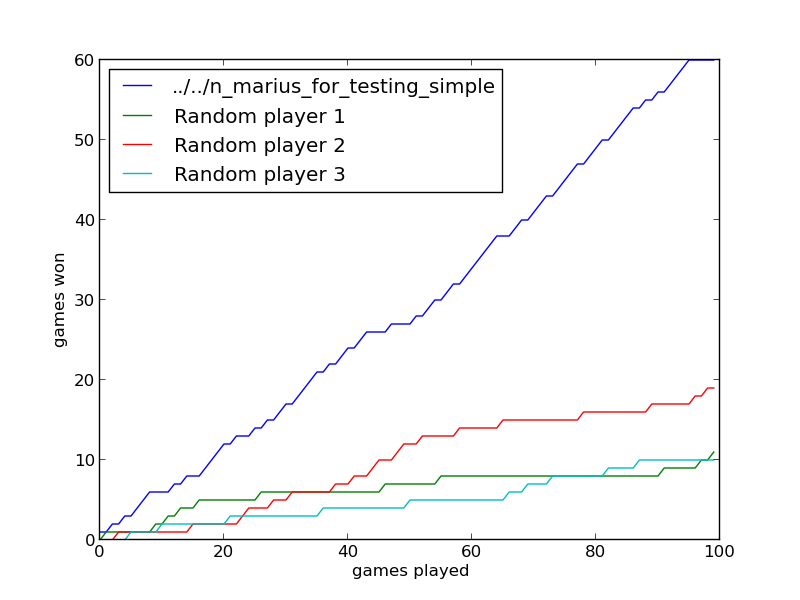
\includegraphics[width=\textwidth]{../marius_25_25_bias_against_random.png}
                \caption{100 games against 3 random opponents.}
                \label{fig:mar1}
        \end{subfigure}%
        ~ %add desired spacing between images, e. g. ~, \quad, \qquad, \hfill etc.
          %(or a blank line to force the subfigure onto a new line)
        \begin{subfigure}[b]{0.35\textwidth}
                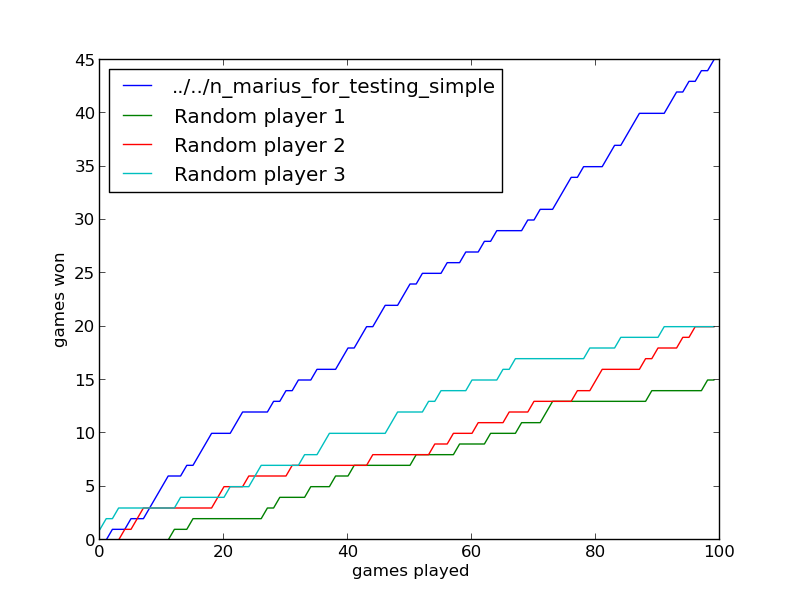
\includegraphics[width=\textwidth]{../marius_25_25_bias_against_random2.png}
                \caption{100 games against 3 random opponents.}
                \label{fig:mar2}
        \end{subfigure}%
        ~ %add desired spacing between images, e. g. ~, \quad, \qquad, \hfill etc.
          %(or a blank line to force the subfigure onto a new line)
        \begin{subfigure}[b]{0.35\textwidth}
                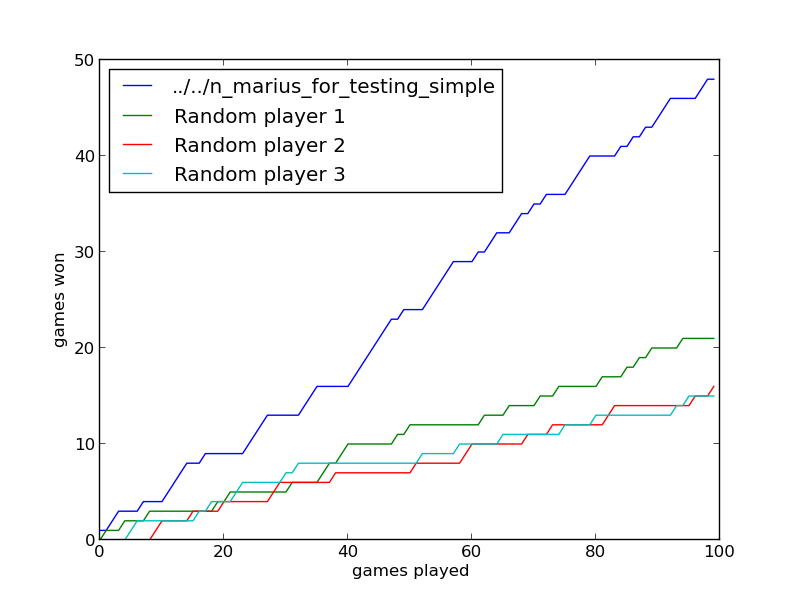
\includegraphics[width=\textwidth]{../marius_25_25_bias_against_random3.png}
                \caption{100 games against 3 random opponents.}
                \label{fig:mar3}
        \end{subfigure}%
        \caption{Results of the agent trained by human input data, playing against random players. The wins for the agent is shown in blue. }\label{fig:marius_training}
\end{figure}


\subsection*{Analysis and Discussion}

It is shown that it is possible to train a network to be able to beat the opponent. Quite a lot of tweaking were required to make the system work. And in some cases it was possible to train the network to be worse than the random player.

%%%%%%%%%%%%%%%%%%%%%%%%%%%%%%%%%%%%%%%%%%%%%%%%%%%%%%%%%%%%%%%%%%%%%%%%%%%%%%%%%

\section*{Randomly Winning}

Though the human trained did perform good it could be interesting to train with a much larger dataset. Another test were performed to test the pack propagations possibility of learning simply from random games. Numerous games were played with random agents and for every game that resulted in a win, states chosen moves were collected for every round. Thus a dataset to win against random agents were created. 

\subsection*{Method} 

To test what network best fitted such data, backpropagation were performed for increasingly larger neural network with along with an increasing number of training epochs. Using this data a player was created to compete against random players.

Using the optimal set of hidden neurons, an ANN was trained for 10 epochs, using a weight of 0.01 and a weight decay of 0.001. As this gave the best results.

\subsection*{Result}

The test for lowest error can be seen in figure \ref{fig:3D}. 

Fitting the data using automatically generated data. Trying to decide the optimal size to fit the data, i.e. the test data.

\begin{figure}[t]
        \centering
		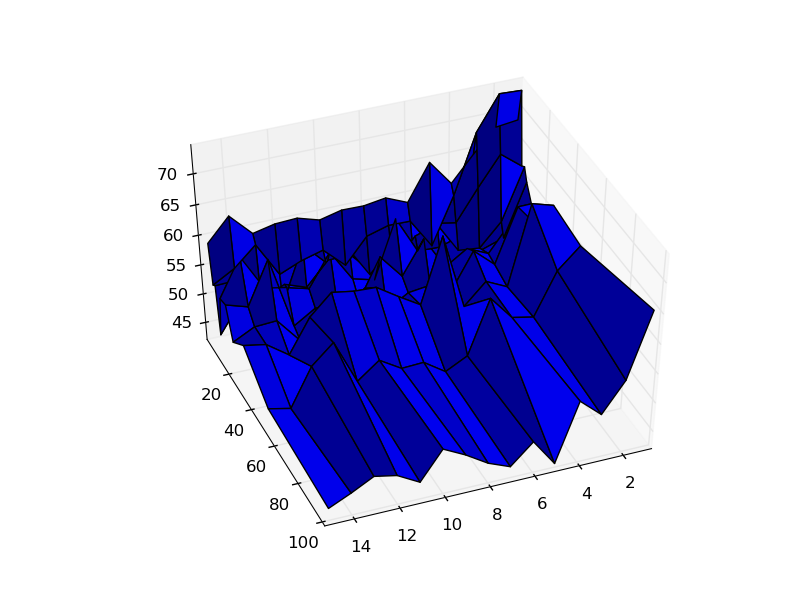
\includegraphics[scale=0.3]{../testing_fit_3D.png} 
        \caption{ Plot showing the error of the training set using different epochs and number of hidden neurons. Respectively on the right and left side.}\label{fig:3D}
\end{figure} 

The result of the randomly generated player against.



\subsection*{Analysis and Discussion}

Not surprisingly the more hidden neurons the better fit can be achieved.

%%%%%%%%%%%%%%%%%%%%%%%%%%%%%%%%%%%%%%%%%%%%%%%%%%%%%%%%%%%%%%%%%%%%%%%%%%%%%%%%%


\section*{Imitating Another Agent}

The problem with imitating the random player is that it is not able to keep a consistent plan. As the backpropagation is trying to minimize the error between input and output. For example when choosing which piece to move from the start after a roll of 6 the random players chose each one randomly. For a neural network it is impossible to imitate this and it would introduce error to the backpropagation fit.

A better idea would be to imitate an agent that uses a consistent plan to win. Multiple agents using GOFAI were created and the QuickPlayer were chosen. The quick player uses a simple greedy approach of always moving the furthest token which can get closets to the goal.

\subsection*{Method}

To be able to predict the player better a much larger neural network were created. 100 games were played and every state and chosen move for the QuickPlayer were chosen. These were used as input for the back propagation. 

Multiple runs with the backpropagation were used running with an momentum of 0.01 and a weight decay of 0.001 as it had to run through the large data set with size 36599. The backpropagation were run for 15 epochs effectively giving an error about 65 \%.

\subsection*{Results}

The results of the training can be seen in figure \ref{fig:quick_training}. Subfigure \ref{fig:qui2} shows the trained network against 3 random opponents. The win ratio is just below 0.5. The effectiveness of the trained network can be seen in subfigure \ref{fig:qui2}. It plays with almost the same effectiveness as the QuickPlayer with a ratio of below 0.5 wins per play. Subfigure \ref{fig:qui3} shows the two agents playing against each other. It can be seen that both QuickPlayers peform a little better than the trained networks.


\begin{figure}
        \centering
        \begin{subfigure}[b]{0.35\textwidth}
                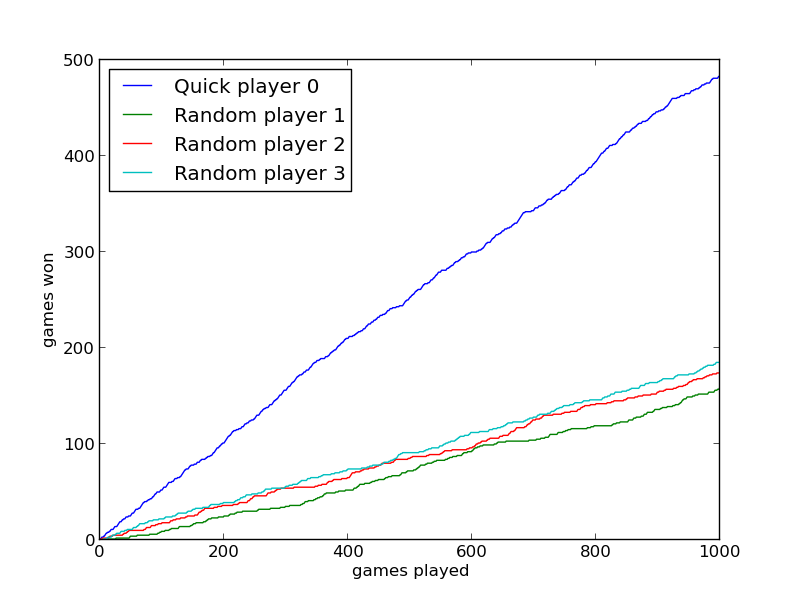
\includegraphics[width=\textwidth]{../training_quick_results.png}
                \caption{Result of 1000 for the QuickPlayer against 3 random opponents. \\ }
                \label{fig:qui1}
        \end{subfigure}%
        ~ %add desired spacing between images, e. g. ~, \quad, \qquad, \hfill etc.
          %(or a blank line to force the subfigure onto a new line)
        \begin{subfigure}[b]{0.35\textwidth}
                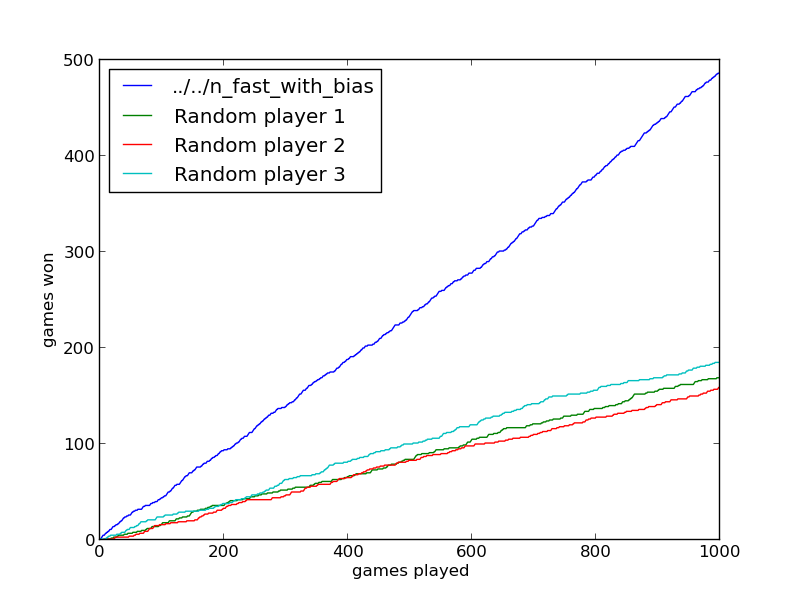
\includegraphics[width=\textwidth]{../training_quick_trained.png}
                \caption{Result of 1000 for the player trained by the QuickPlayers moves against 3 random opponents.}
                \label{fig:qui2}
        \end{subfigure}%
        ~ %add desired spacing between images, e. g. ~, \quad, \qquad, \hfill etc.
          %(or a blank line to force the subfigure onto a new line)
        \begin{subfigure}[b]{0.35\textwidth}
                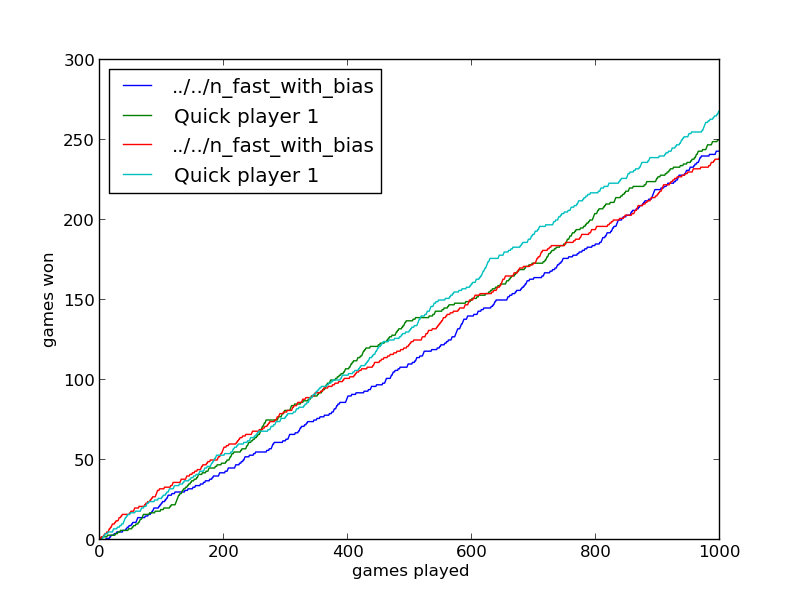
\includegraphics[width=\textwidth]{../training_quick_vs_trained.png}
                \caption{1000 games of two QuickPlayers against two trained networks. \\}
                \label{fig:qui3} 
        \end{subfigure}%
        \caption{The QuickPlayer against the trained ANN player }\label{fig:quick_training}
\end{figure}



\subsection*{Analysis and Discussion}

Figure \ref{fig:qui2} shows very promising results towards training the network. Though the QuickPlayer is a very simple agent to train against. Especially because it is simply dependent on which token can move to the furthest position. Thus if the bias is set so that it simply returns the same set of results every time the effect would be the same as bringing one player to the goal. When the player moves into the goal the agent would chose the token with the second best score. Effectively making it use the same strategy as the QuickPlayer, which could explain why it is able to play on equal terms. And when the ANN is trained towards this it would be very hard to correct this.

%%%%%%%%%%%%%%%%%%%%%%%%%%%%%%%%%%%%%%%%%%%%%%%%%%%%%%%%%%%%%%%%%%%%%%%%%%%%%%%%%


\section*{Random Neural Networks}

It was seen that the trained networks did perform better than the random players. Though to test that this is actually the result of training, the effectiveness of simply using neural networks are to be tested. That is, how does any agent using randomly generated weights perform against random players.

\subsection*{Method}

The network was made with a hidden layer of size 5 with no bias. They were made to be simple as the weight were random \footnote{why exactly} Parameters were randomly generated with values between -1 and 1.  50 different neural networks playing against three random players for 100 games. 

\subsection*{Results}

The results of the multiple agents games can be seen in figure \ref{fig:random_50}. Only in one of the games is the number of wins less than 25. The mean of multiple of such simulations never went below 40 wins.

\begin{figure}[t]
        \centering
		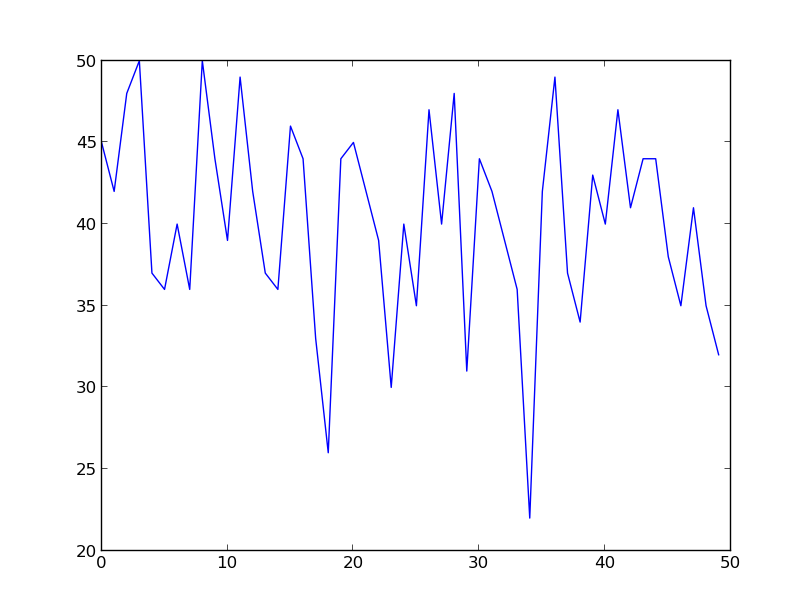
\includegraphics[scale=0.3]{../50_random_1.png} 
        \caption{ Number of wins for 100 ludo games for 50 different randomly generated neural networks. }\label{fig:random_50}
\end{figure} 

\subsection*{Analysis and Discussion}

It can be seen simply having a plan makes the network better. It is possible that the scaling of inputs between  -1 and 1 did have an effect in making the parameters good. Though most likely it simply stems from the fact that moving more consistently, when possible, is a better strategy than moving random. 

%%%%%%%%%%%%%%%%%%%%%%%%%%%%%%%%%%%%%%%%%%%%%%%%%%%%%%%%%%%%%%%%%%%%%%%%%%%%%%%%%

\section*{Number of valid moves}

It was seen that even a randomly generated network gives a good performance against the random player. It is thus of interest to see what kind of moves is actually returned from the neural network. That is does it give valid moves and is there any difference towards different input.

\subsection*{Method}

To test the valid moves 100 games are played and every time the agent makes a move the ANN's priority of this move is checked. To check the consistency of the ANN 1000 different states are sampled and the output is compared.

\subsection*{Results}

For the human and QuickPlayer trained networks the ratio of valid moves were 0.332 and 0.325 respectively. Testing the 1000 randomly generated input between 0 and 1 gave the completely same result. I.e. for the QuickPlayer generated the output was [ 0.30486155  0.31426025  0.33858957  0.04048108] and for the human trained the output was [ 0.36656972  0.334266    0.06157172  0.23690873].

\subsection*{Analysis and Discussion}

From the randomly generated data input it is seen that the trained networks simply are a clone of the QuickPlayer. Thus no actual choices are made as the bias simply overrules the input. Effectively the ANN's are simply 'dead' networks with no reaction.


%%%%%%%%%%%%%%%%%%%%%%%%%%%%%%%%%%%%%%%%%%%%%%%%%%%%%%%%%%%%%%%%%%%%%%%%%%%%%%%%%


\section*{Playing against other Agents}

To test the effectiveness of the trained players another LUDO player was borrowed from Leon Larsen. This agent is also trained but does use quite a different approach. 


It makes sense that it is very hard to fit actually some of random players .

Leons agent. Trained sequentially with preprocessed input.

The input to the network is as follows.


Reinforcement learning.

\subsection*{Results}

The results of the training can be seen in figure \ref{fig:quick_training}. Subfigure \ref{fig:qui2} shows the trained network against 3 random opponents. The win ratio is just below 0.5. The effectiveness of the trained network can be seen in subfigure \ref{fig:qui2}. It plays with almost the same effectiveness as the QuickPlayer with a ratio of below 0.5 wins per play. Subfigure \ref{fig:qui3} shows the two agents playing against each other. It can be seen that both QuickPlayers peform a little better than the trained networks.


\begin{figure}
        \centering
        \begin{subfigure}[b]{0.5\textwidth}
                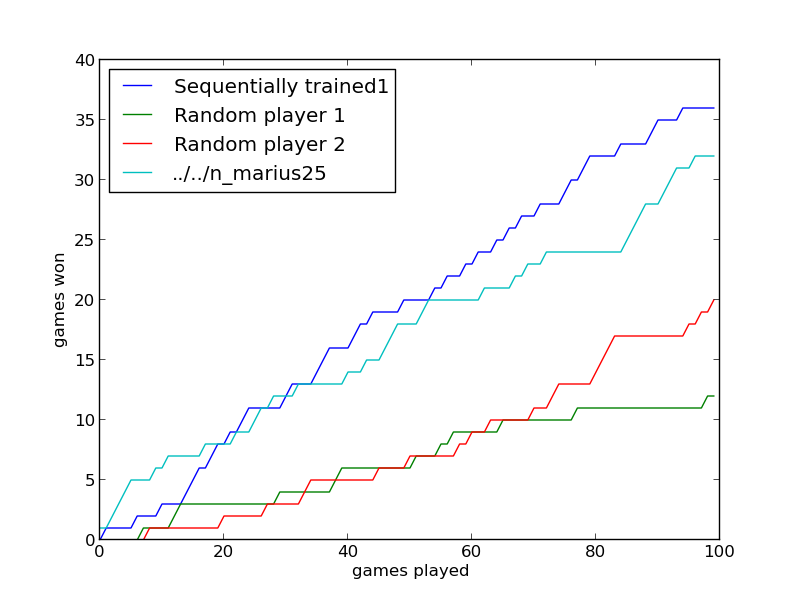
\includegraphics[width=\textwidth]{../against_leo_mar.png}
                \caption{Result of 100 for the player trained against the Sequentially trained and 2 random opponents.}
                \label{fig:vle1}
        \end{subfigure}%
        ~ %add desired spacing between images, e. g. ~, \quad, \qquad, \hfill etc.
          %(or a blank line to force the subfigure onto a new line)
        \begin{subfigure}[b]{0.5\textwidth}
                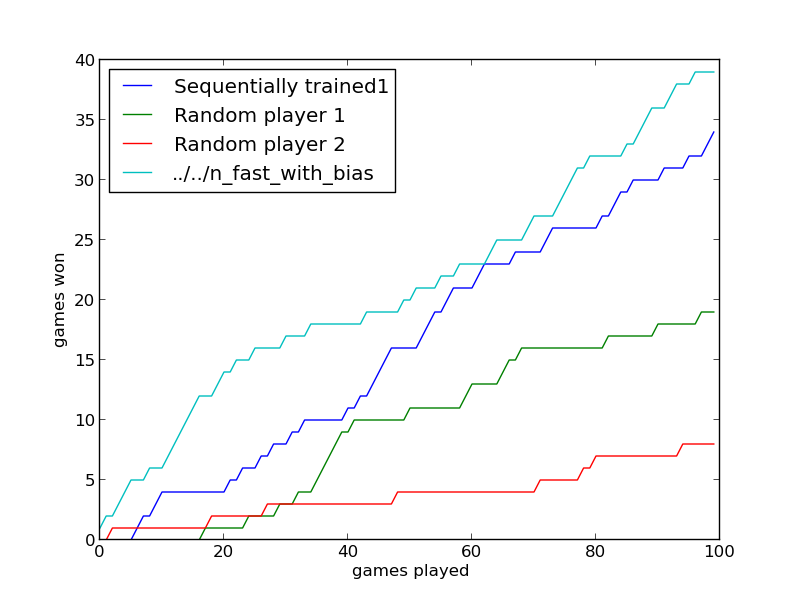
\includegraphics[width=\textwidth]{../against_leo_qui.png}
                \caption{Result of 100 for the network trained towards QuickPlayer against the Sequentially trained and 2 random opponents.}
                \label{fig:vle2}
        \end{subfigure}%
        \caption{ Results of the two trained networks against the best performing sequential network. }\label{fig:against_seq}
\end{figure}


\subsection*{Analysis and Discussion}


From the initial generation of datasets with random parameters it can be seen that all most all of them outperform the random approach. This indicates that using somewhat of a plan will outperform a completely random approach. Though testing of the trained players showed that the ANN didn't respond to any of the input, but simply relied on the fact that if the desired output wasn't possible the second best would be chosen.

Though the effect of this approach especially against the Sequentially trained player. 


\section*{Conclusion} % 5%

Using the backpropagation to copy the advanced players does not seem to be able to work. The number of and shape could of course have been completely wrong. 

Another interesting result is the effectiveness of using a consistent plan for the LUDO player. Even though the 
ANN networks effectively didn't make any choices based on the input. 

And interesting results were also seen from the fight against the Sequential Player. It was actually outperformed by the ANN simply trained by the QuickPlayer. This gives an idea about the complexity of the LUDO game as a simple "dead" player could outperform the active player using preprocessed input. Though being able to train against the ANN trained by the QuickPlayer the Sequential could possibly outperform it drastically.

The complete set of states is a very large input. It was simply to complicated for the backpropagation to find any consistency when using the given ANN size. Preprocessing the input could drastically reduce the input size and complexity thus making it much easier to find consistency. \cite{frean:mar} was avoided because of the complexity of the LUDO input. Though given proper preprocessed data this would be an interesting approach to build components to determine the fitness of moves.

%%% Dette lyder meget st�rkt, skal skrives om

The tests gives an insight into the limits of artificial neural networks. To be able to train the networks properly one needs to have a proper insight to the system designing the network for. One needs to chose proper parameters as input if the network should be able find any consistency. Thus the black box approach for training ANN seems very infeasible. \cite{chellapilla:k} shows that using proper preprocessing it is possible to solve the LUDO problem quite effectively using neural networks thus indicating that this should also be the case for the implementation of LUDO.

%%
It could be very interesting to test the ability to train towards GOFAI players using other approaches with the input preprocessed towards their solution. Possibly starting with a more simple version of the game to determine how to preprocess the data and determine the effectiveness of different setups.



\section*{Acknowledgements} %5

Marius Hagelskjaer, my little brother, for sitting through and judging more than 200 different ludo states. \\

\noindent Leon Larsen, for providing the sequential LUDO player to play against. \\

\noindent The simulator was developed in shared effort with Rudi Hansen, Leon Larsen and Kent Stark Olsen.
\begin{thebibliography}{[MT1]}
%

\bibitem[IC]{NeuronOnline}
\url{http://www.doc.ic.ac.uk/~nd/surprise_96/journal/vol4/cs11/report.html}
May (2014)
%
\bibitem[LU]{LudoWiki}
\url{http://en.wikipedia.org/wiki/Ludo_%28board_game%29}
May (2014)

\bibitem[AI2]{Russell}
Russell, S. J. and Norvig, P.
Artificial Intelligence: A Modern Approach
2. Edition
Pearson Education (2010)
%
\bibitem[SR1]{schaul2010}
Schaul, T. and Bayer, J. and Wierstra, D. and Sun, Y. and Felder, M. and Sehnke, F. and R\"{u}ckstie\ss, T. and Schmidhuber, J.
PyBrain
Journal of Machine Learning Research (2010)
%
\bibitem[DR1]{Rumelhart}
Rumelhart, D. E. and Hinton, G. E. and Williams, R. J.
Learning Representations by Back-propagating Errors
Neurocomputing: Foundations of Research 696--699 (1988)
%
\bibitem[FA1]{ludoanalysis}
Alvi, F. and Ahmed, M.
Complexity analysis and playing strategies for Ludo and its variant race games
Computational Intelligence and Games (CIG), 2011 IEEE Conference on 134-141 (2011)
%
\bibitem[FM1]{frean:mar}
Frean, M.
The upstart algorithm: A method for constructing and training feedforward neural networks
Neural Computation 2, 198-209 (1990)
%
\bibitem[KC1]{chellapilla:k}
Chellapilla, K. and Fogel, D.B.
Evolution, neural networks, games, and intelligence
Proceedings of the IEEE , vol.87, no.9, 1471 - 1496 Sep(1999)


\end{thebibliography}


\end{document}
